\section{Experiments} \label{sec:exp}

A prototype version of {\FORPI} has been implemented in the functional programming language Scala as part of the \skeptik
library. This library includes an implementation of {\GFOLU} \cite{GFOLU}. In order to evaluate the algorithm's effectiveness, {\FORPI} was tested on two data sets: proofs generated by a real theorem prover and randomly-generated resolution proofs. The proofs are included in the source code repository, available at \url{https://github.com/jgorzny/Skeptik}. Note that by implementing the algorithms in this library, we are able to guarantee the correctness of the compressed proofs, as in \skeptik every inference rule (e.g. resolution, contraction) is implemented as a small class (at most 178 lines of code) with a constructor that checks whether the conditions for the application of the rule are met, thereby preventing the creation of objects representing incorrect proof nodes (i.e. unsound inferences). With logical soundness guaranteed by \skeptik's data structures, to ensure the soundness of a proof compression algorithm, we only need to check that the root clause of the compressed proof is equal to or stronger than the root clause of the input proof and that the set of axioms used in the compressed proof is a (possibly non-proper) subset of the set of axioms used in the input proof.

%Note: the 178 class size is for the class  definition only. Not including the object, or other code defined in those files (e.g. traits). With object lines counted as well, the value is 199. The largest is contraction

%\footnote{Source code available at \url{https://github.com/jgorzny/Skeptik}} %note: removed footnote because journal says footnotes should be avoided if possible,

First, {\FORPI} was evaluated on the same proofs used to evaluate {\GFOLU}. These proofs were generated by executing the {\SPASS} theorem prover ({\url{http://www.spass-prover.org/}) on 1032 real-world unsatisfiable first-order problems without equality from the TPTP Problem Library \cite{TPTP}. In order to generate pure resolution proofs, the advanced inference rules of {\SPASS} were disabled. The proofs were originally generated on the Euler Cluster at the University of Victoria with a time limit of 300 seconds per problem. Under these conditions, {\SPASS} was able to generate 308 proofs. The proofs generated by {\SPASS} were small: proof lengths varied from 3 to 49, and the number of resolutions in a proof ranged from 1 to 32.

%Note that the proofs were not re-generated for the TPTP data?


In order to test {\FORPI}'s effectiveness on larger proofs, a total of 2280 proofs were randomly generated and then used as a second benchmark set. The randomly generated proofs were much larger than those of the first data set: proof lengths varied from 95 to 700, while the number of resolutions in a proof ranged from 48 to 368.
Proofs were generated by the following procedure: start with a root node whose conclusion is $\bot$, and make two premises $\eta_1$ and $\eta_2$ using a randomly generated literal such that the desired conclusion is the result of resolving $\eta_1$ and $\eta_2$. For each node $\eta_i$, determine the inference rule used to make its conclusion: with probability $p=0.9$, $\eta_i$ is the result of a resolution, otherwise it is the result of a contraction. 
Literals are generated by uniformly choosing a number from $\{1,\dots,k,k+1\}$ where $k$ is the number of predicates generated so far; if the chosen number $j$ is between $1$ and $k$, the $j$-th predicate is used; otherwise, if the chosen number is $k+1$, a new predicate with a new random arity (at most four) is generated and used. Each argument is a constant with probability $p=0.7$ and a complex term (i.e. a function applied to other terms) otherwise; functions are generated similarly to predicates. 
If a node $\eta$ should be the result of a resolution, then with probability $p=0.2$ we generate a left parent $\eta_\ell$ and a right parent $\eta_r$ for $\eta$ (i.e. $\eta = \eta_\ell \odot \eta_r$) having a common parent $\eta_c$ (i.e. $\eta_l = (\eta_\ell)_\ell \odot \eta_c$ and $\eta_r = \eta_c \odot (\eta_r)_r$, for some newly generated nodes $(\eta_\ell)_\ell$ and $(\eta_r)_r$ ). The common parent ensures that also non-tree-like DAG proofs are generated. This procedure is recursively applied to the generated parent nodes. 
Each parent of a resolution has each of its terms not contained in the pivot replaced by a fresh variable with probability $p=0.7$.
At each recursive call, the additional minimum height required for the remainder of the branch is decreased by one with probability $p=0.5$. Thus if each branch always decreases the additional required height, the proof has height equal to the initial minimum value. The process stops when every branch is required to add a subproof of height zero or after a timeout is reached. In any case, the topmost generated node for each branch is generated as an axiom node. The minimum height was set to 7 (which is the minimum number of nodes in an irregular proof plus one) and the timeout was set to 300 seconds (the same timeout allowed for {\SPASS}). The probability values used in the random generation were carefully chosen to produce random proofs similar in shape to the real proofs obtained by {\SPASS}. For instance, the probability of a new node being a resolution (respectively, contraction) is approximately the same as the frequency of resolutions (respectively, contractions) observed in the real proofs produced by {\SPASS}.


For consistency, the same system and metrics were used. Proof compression and proof generation was performed on a laptop (2.8GHz Intel Core i7 processor with 4GB of RAM (1333MHz DDR3) available to the Java Virtual Machine). For each proof $\psi$, we measured the time needed to compress the proof ($t(\psi)$) and the compression ratio ($(|\psi|-|\alpha(\psi)|)/|\psi|$) where $|\psi|$ is the number of resolutions in the proof, and $\alpha(\psi)$ is the result of applying a compression algorithm or some composition of {\FORPI} and {\GFOLU}. Note that we consider only the number of resolutions in order to compare the results of these algorithms to their propositional variants (where contractions are implicit). Moreover, contractions could be made implicit within resolution inferences even in the first-order case and we use explicit contractions only for technical convenience.

%\begin{figure}[bt]
%\centering
%  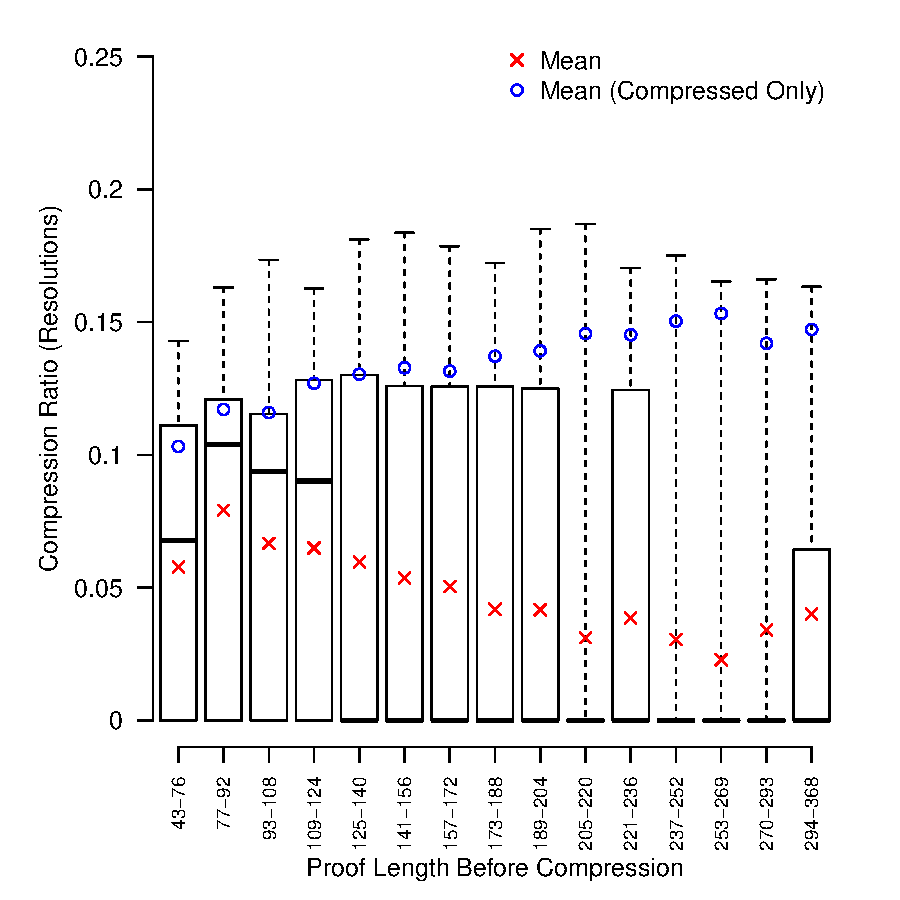
\includegraphics[scale=0.5]{images/final-random-forpi-compress_ratio_res_vs_proof_res_length.pdf}  
%    \caption{Compression Ratio (\FORPI)}
%    \label{fig:forpimean}
%    \end{figure}
%Figure \ref{fig:forpimean} shows a box-whisker plot of compression ratio with proofs grouped by number of resolutions and whiskers indicating a minimum and maximum compression ratio achieved within the group. The circles indicate the mean compression ratio when considering only proofs for which some compression was achieve, and these points indicate that when larger proofs can be compressed, they are compressed more than smaller proofs.



\begin{table*}[bt]
\centering
\begin{tabular}{| l || r | r | r || r | r | r  | }
\hline
 Algorithm& \multicolumn{3}{c ||}{\# of Proofs Compressed} & \multicolumn{3}{c |}{\# of Removed Nodes}  \\
& \multicolumn{1}{c }{TPTP} & \multicolumn{1}{c}{Random}  & \multicolumn{1}{c ||}{Both}  & \multicolumn{1}{c }{TPTP} & \multicolumn{1}{c }{Random} & \multicolumn{1}{c |}{Both}  \\ \hline \hline
{\GFOLU}(p) & 55 (17.9\%) & 815 (35.7\%) & 870 (33.6\%)  & 107 (4.8\%) & 17,730 (4.5\%) & 17,837 (4.5\%)    \\ \hline
{\FORPI}(p)  & 11 (3.6\%) &  252 (11.1\%) & 263 (10.2\%)  &  13 (0.6\%) &  15,913 (4.0\%) & 15,926 (4.0\%)   \\ \hline
{\GFOLU}({\FORPI}(p))   & 55 (17.9\%) & 993 (43.6\%) & 1048 (40.5\%) & 108 (4.8\%)  & 33,956 (9.1\%) & 34,064 (9.1\%) \\ \hline
{\FORPI}({\GFOLU}(p)) & 11 (3.6\%) & 993  (43.6\%)&  1004 (38.8\%) & 108 (4.8\%) & 36,070 (9.1\%) & 36,178 (9.1\%)  \\ \hline
Best                            & 56 (18.2\%) & 993 (43.6\%) & 1049 (40.5\%)   & 108 (4.8\%) & 39,742 (10.1\%) & 39,850 (10.1\%)     \\ \hline
\end{tabular}
\vspace{5pt}
\caption{Number of proofs compressed and number of overall nodes removed}
\label{tab:results}
\end{table*}




\begin{table*}[bt]
\centering
\begin{tabular}{| l | r | r || l | r |}
\hline
Algorithm &  \multicolumn{2}{c ||}{First-Order Compression}  &  Algorithm & Propositional Compression \cite{Boudou}  \\
& $~~~~$ All   & Compressed Only & & \\ \hline \hline
{\GFOLU}(p) &  3.4\%& 33.1\% &{\LU}(p) & 7.5\% \\ \hline
{\FORPI}(p) & 4.5\%&  13.4\%&{\RPI}(p) &  17.8\% \\ \hline
{\GFOLU}({\FORPI}(p)) &  7.6\%& 19.7\%& ({\LU}({\RPI}(p)) &  21.7\% \\ \hline
{\FORPI}({\GFOLU}(p)) &  8.1\%& 21.0\%& ({\RPI}({\LU}(p)) & 22.0\% \\ \hline
Best & 9.2\% & 22.8\%&  Best &  22.0\% \\ \hline
\end{tabular}
\vspace{5pt}
\caption{Mean compression results}
\label{tab:result-mean}
\end{table*}

Table \ref{tab:results} summarizes the results of {\FORPI} and its combinations with {\GFOLU}. The first set of columns describes the percentage of proofs that were compressed by each compression algorithm. The algorithm `Best' runs both combinations of {\GFOLU} and {\FORPI} and returns the shortest proof output by either of them. The total number of proofs is $308+2280=2588$ and the total number of resolution nodes is $2,249 + 393,883
= 396,132$. The percentages in the last three columns are computed by $(\Sigma_{\psi \in \Psi} |\psi|  - \Sigma_{\psi\in \Psi} |\alpha(\psi)|)/(\Sigma_{\psi \in \Psi} |\psi|)$ for each data set $\Psi$ (TPTP, Random, or Both). The use of {\FORPI} alongside {\GFOLU} allows at least an additional 5\% of proofs to be compressed. Furthermore, the use of both algorithms removes more than twice as many nodes than any single algorithm.
%Only nine proofs from the TPTP data set were compressed by {\FORPI}, reducing the number of resolutions by at least one and at most three. However, 252 (0.11\%) of the randomly generated proofs achieved some compression using only {\FORPI}.
%{\FORPI} was able to achieve an overall average compression ratio 5\% on this data. The compression ratio for only the compressed proofs is 33\%, compared to 13\% for {\GFOLU}.

Table \ref{tab:result-mean} compares the results of {\FORPI} and its combinations with {\GFOLU} with their propositional variants as evaluated in  \cite{Boudou}. The first column describes the mean compression ratio for each algorithm including proofs that were not compressed by the algorithm, while the second column calculates the mean compression ratio considering only compressed proofs. It is unsurprising that the first column is lower than the propositional mean for each algorithm: there are stricter requirements to apply these algorithms to first-order proofs. In particular, additional properties must be satisfied before a unit can be lowered, or before a pivot can be recycled. On the other hand, when first-order proofs are compressed, the compression ratios are on par with or better than their propositional counterparts.

\begin{figure*}[p]
    
  \subfloat[Number of (non-)compressed proofs]{{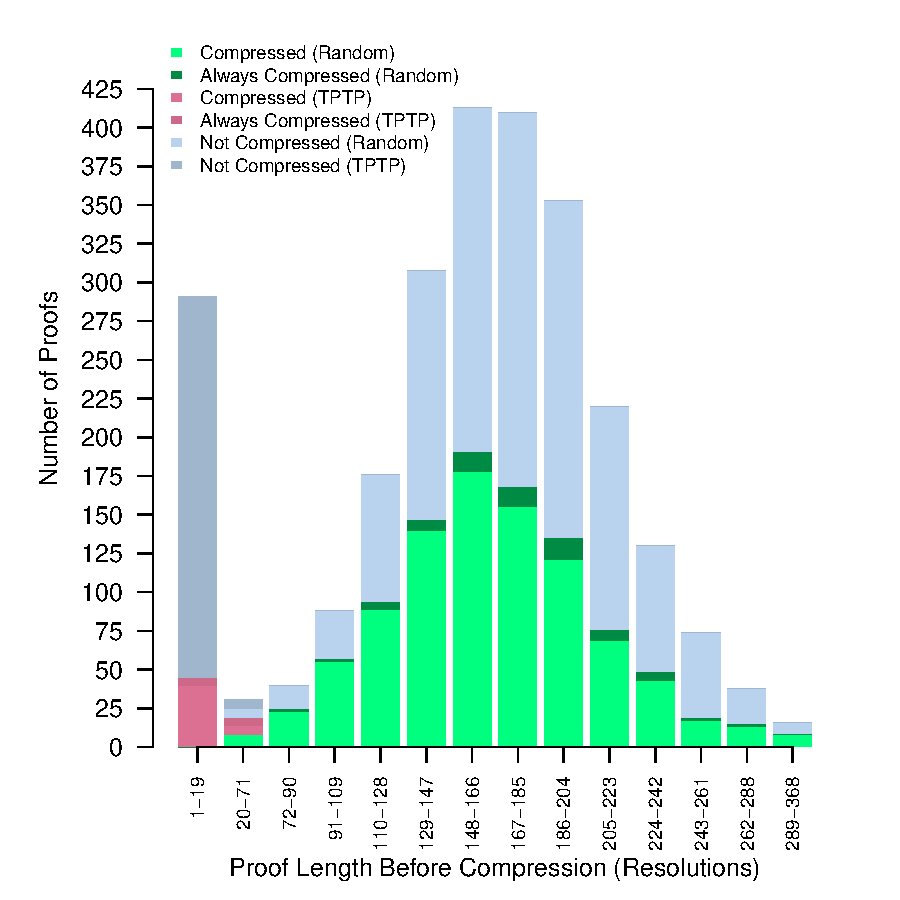
\includegraphics[scale=0.5]{images/combined-all-num_compressed_stacked.pdf} }}
   \subfloat[Compressed length against input length]{{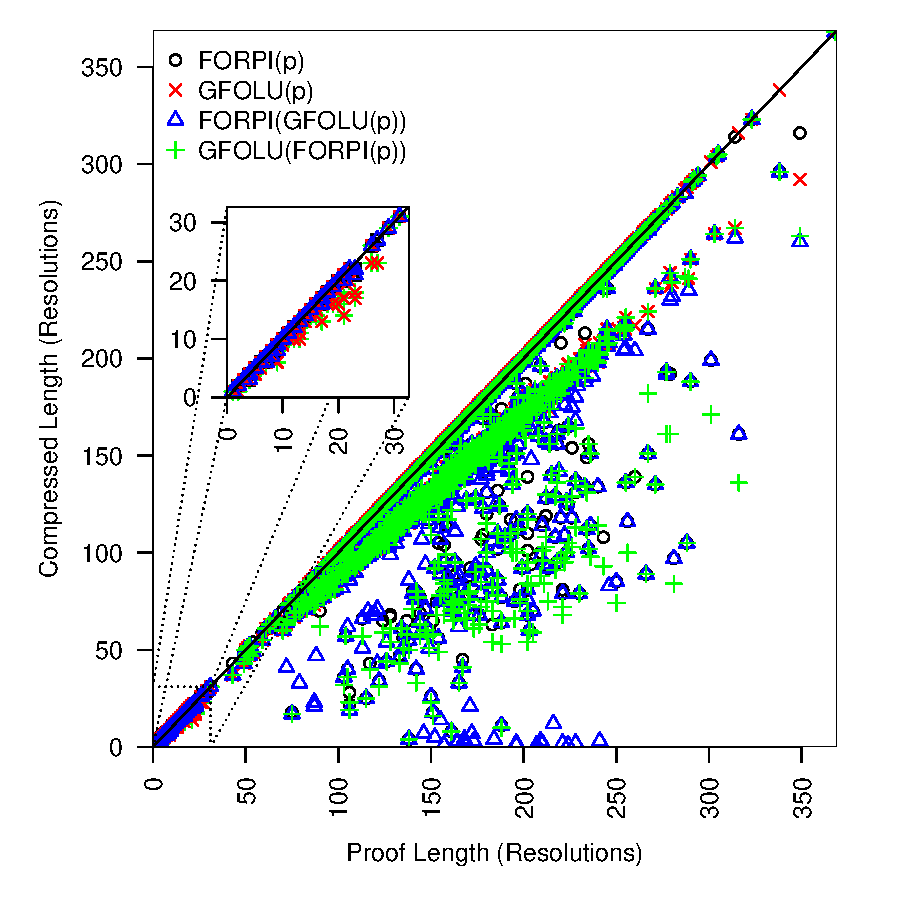
\includegraphics[scale=0.5]{images/combined-all-res-length-vs-compressed-res-length.pdf} }}   
   
\subfloat[\FORPI(\GFOLU(p)) vs. \GFOLU(\FORPI(p))]{{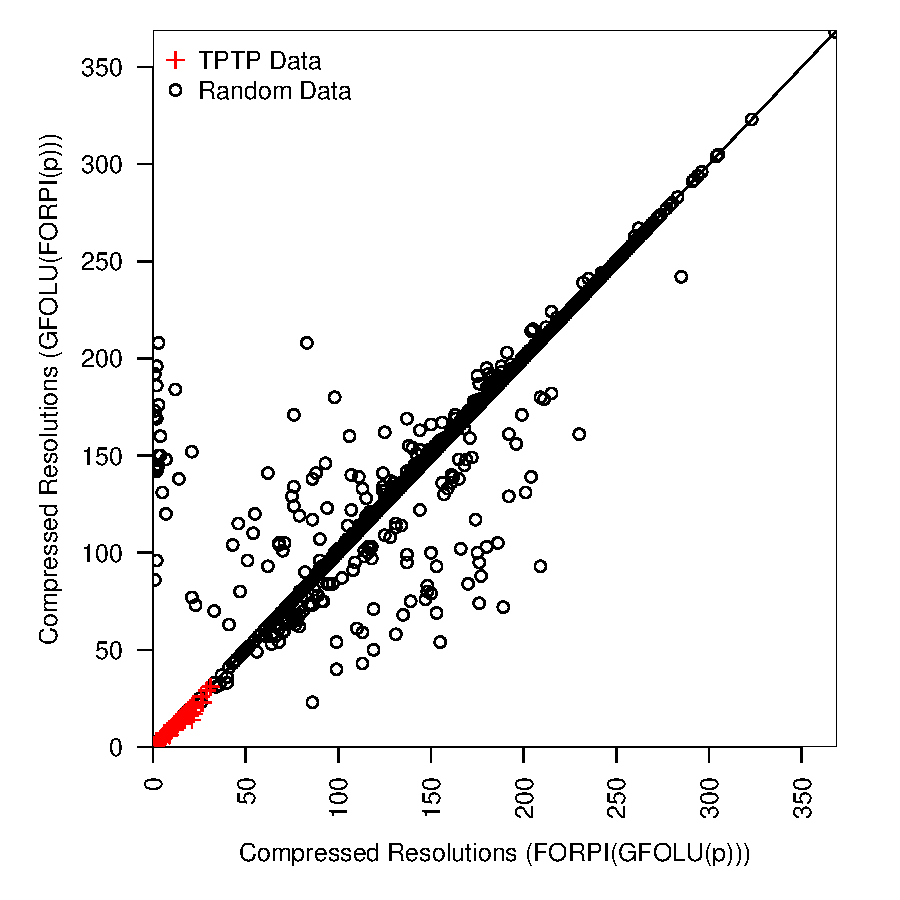
\includegraphics[scale=0.5]{images/combined-alg-res.pdf} }}
  \subfloat[Cumulative proof compression]{{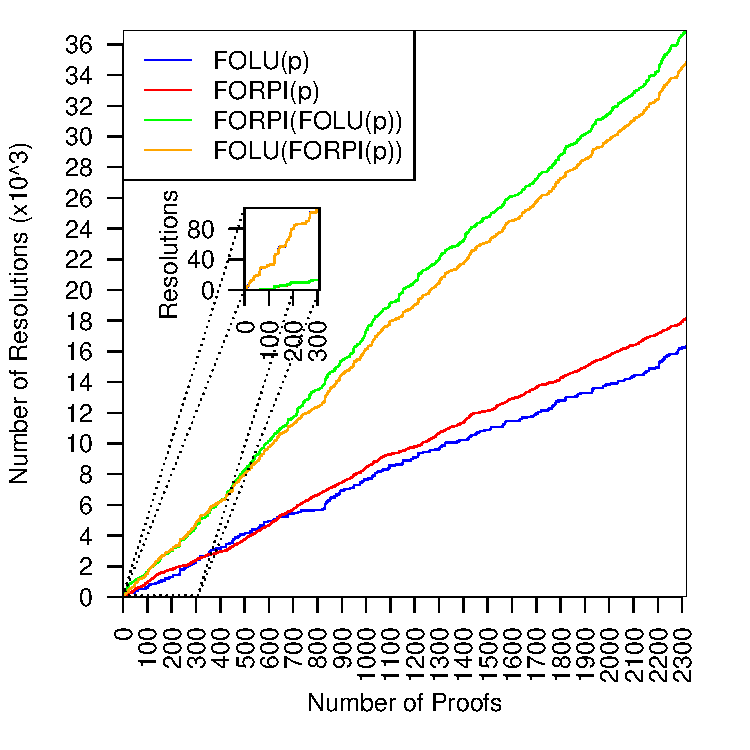
\includegraphics[scale=0.5]{images/combined-all-cumulative-res-nodes-diff.pdf} }}   


 \caption{\GFOLU \& \FORPI Combination Results}
\label{fig:ex}

\end{figure*}

Figure \ref{fig:ex} (a) shows the number of proofs (compressed and uncompressed) per grouping based on number of resolutions in the proof. The red (resp. dark grey) data shows the number of compressed (resp. uncompressed) proofs for the TPTP data set, while the green (resp. light grey) data shows the number of compressed (resp. uncompressed) proofs for the random proofs. The number of proofs in each group is the sum of the heights of each coloured bar in that group. The overall percentage of proofs compressed in a group is indicated on each bar. Dark colors indicate the number of proofs compressed by {\FORPI}, {\GFOLU}, and both compositions of these algorithms; light colors indicate cases were {\FORPI} succeeded, but at least one of {\GFOLU} or a combination of these algorithms achieved zero compression. 
Given the size of the TPTP proofs, it is unsurprising that few are compressed: small proofs are a priori less likely to contain irregularities. On the other hand, 
at least 25\% of randomly generated proofs in each size group could be compressed.
%at least one in four randomly generated proofs could be compressed. 
%\marginpar{TODO: ``at least one in four'' --> I find it hard to conclude this from figure (a). Maybe this statement could be clarified or made more precise.}

%The random proofs indicate that many proofs are irregular, but this is not reflected in the TPTP data; this is unsurprising given the size of the proofs in the TPTP data set.

Figure \ref{fig:ex} (b) is a scatter plot comparing the number of resolutions of the input proof against the number of resolutions in the compressed proof for each algorithm. The results on the TPTP data are magnified in the sub-plot. For the randomly generated proofs (points outside of the sub-plot), it is often the case that the compressed proof is significantly shorter than the input proof. Interestingly, {\GFOLU} appears to reduce the number of resolutions by a linear factor in many cases. This is likely due to a linear growth in the number of non-interacting irregularities (i.e. irregularities for which the lowered units share no common literals with any other sub-proofs), which leads to a linear number of nodes removed.

%\marginpar{TODO: not sure we should keep this impressive example. Isn't it just an outlier? Could it occur in reality? Or is it just a spurious example resulting from the random generation?}
%In some cases, {\FORPI} is able to reduce the number of resolutions by several orders of magnitude, e.g. one proof is reduced from 196 contractions to only 2. 

Figure \ref{fig:ex} (c) is a scatter plot comparing the size of compression obtained by applying {\FORPI} before {\GFOLU} versus {\GFOLU} before {\FORPI}. Data obtained from the TPTP data set is marked in red; the remaining points are obtained from randomly generated proofs. Points that lie on the diagonal line have the same size after each combination. There are 165 points beneath the line and 258 points above the line. Therefore, as in the propositional case \cite{LURPI}, it is not a priori clear which combination is better. Nevertheless, the distinctly greater number of points above the line suggests that it is more often the case that {\FORPI} should be applied after {\GFOLU}. Not only this combination is more likely to maximize the likelihood of compression, but the achieved compression also tends to be larger.

Figure \ref{fig:ex} (d) shows a plot comparing the difference between the cumulative number of resolutions of the first $x$ input proofs and the cumulative number of resolutions in the first $x$ proofs after compression (i.e. the cumulative number of \emph{removed} resolutions). The TPTP data is displayed in the sub-plot; note that the lines for everything except {\FORPI} largely overlap (since the values are almost identical; cf. Table \ref{tab:results}). Observe that it is always better to use both algorithms than to use a single algorithm. The data also shows that using {\FORPI} after {\GFOLU} is normally the preferred order of composition, as it typically results in a greater number of nodes removed than the other combination. An even better approach is to try both combinations and choose the best result (as shown in the `Best' curve).  


{\SPASS} required approximately 40 minutes of CPU time (running on a cluster) to generate all the 308 TPTP proofs. The total time to apply both {\FORPI} and {\GFOLU} on all these proofs was just over 8 seconds on a simple laptop computer. The random proofs were generated in 70 minutes, and took approximately 453 seconds (or 7.5 minutes) to compress, both measured on the same computer.
All times include parsing time. These compression algorithms continue to be very fast in the first-order case, and may simplify the proof considerably for a relatively small cost in time.

%the compression obtained by applying {\FORPI} and {\GFOLU} (as well as their combinations) to the proofs. 
%Unsurprisingly, applying both algorithms generally does better than either algorithm alone. 
%With this data set, {\FORPI} compresses a few proofs only, and its performance is not as good as that of {\GFOLU}. Furthermore, when {\FORPI} is combined with {\GFOLU}, {\FORPI} provides additional compression to only three proofs already compressed by {\GFOLU}. This is surprising, because in the propositional case, {\RPI} usually compresses up to ten times more than {\LowerUnits}. Nevertheless, this can be easily explained by the fact that all available benchmark proofs have small heights (not more than 11); consequently the path from any node to the root is short and unlikely to contain irregularities. In the propositional case, on the other hand, {\RPI} has been tested on proofs that are a thousand times higher.





% although more data is needed for confirmation. The number of points above and below the main diagonal are the same; however, the points below may simply be the result of {\GFOLU} being more likely to compress such short proofs. If so, that would imply that running {\FORPI} after {\GFOLU} is more successful, which would be consistent with propositional results for these algorithms.
%Running {\FORPI} after {\GFOLU} shows some compression that...
%This is consistent with propositional results for these algorithms.

%Before evaluating this algorithm, we first generated several benchmark proofs. This was done by executing the {\SPASS}\footnote{\url{http://www.spass-prover.org/}} theorem prover on 2280 real first-order problems without equality of the TPTP Problem Library \footnote{\url{http://www.cs.miami.edu/{\textasciitilde}tptp/}} (among them, 1032 problems are known to be unsatisfiable). In order to generate pure resolution proofs, most advanced inference rules used by {\SPASS}  were disabled. The Euler Cluster at the University of Victoria\footnote{\url{https://rcf.uvic.ca/euler.php}} was used and the time limit was 300 seconds per problem. Under these conditions, {\SPASS} was able to generate 308 proofs. 


%The proofs generated by {\SPASS} were small (with lengths from 3 to 49). These proofs are specially small in comparison with the typical proofs generated by SAT- and SMT-solvers, which usually have from a few hundred to a few million nodes. The number of proofs (compressed and uncompressed) per length is shown in Figure \ref{fig:ex} (b). Uncompressed proofs are those which had either no lowerable units to lower or for which \SFOLowerUnits failed and returned the original proof. Such failures occurred on only 14 benchmark proofs. Among the smallest of the 308 proofs, very few proofs were compressed. This is to be expected, since the likelihood that a very short proof contain a lowerable unit (or even merely a unit with more than one child) is low. The proportion of compressed proofs among longer proofs is, as expected, larger, since they have more nodes and it is more likely that some of these nodes are lowerable units. 13 out of 18 proofs with length greater than or equal to 30 were compressed. 

%Figure \ref{fig:ex} (a) shows a box-whisker plot of compression ratio with proofs grouped by length and whiskers indicating minimum and maximum compression ratio achieved within the group. Besides the median compression ratio (the horizontal thick black line), the chart also shows the mean compression ratios for all proofs of that length and for all compressed proofs (the red cross and the blue circle). In the longer proofs (length greater than 34), the median and the means are in the range from 5\% to 15\%, which is satisfactory in comparison with the total compression ratio of 7.5\% that has been measured for the propositional {\LowerUnits} algorithm on much longer propositional proofs \cite{Boudou}.

%Figure \ref{fig:ex} (c) shows a scatter plot comparing the length of the input proof against the length of the compressed proof. For the longer proofs (circles in the right half of the plot), it is often the case that the length of the compressed proof is significantly lesser than the length of the input proof.

%Figure \ref{fig:ex} (d) plots the cumulative original and compressed lengths of all benchmark proofs (for an x-axis value of $k$, the cumulative curves show the sum of the lengths of the shortest $k$ input proofs). The total cumulative length of all original proofs is 4429 while the cumulative length of all proofs after compression is 3929. This results in a total compression ratio of 11.3\%, which is impressive, considering that the inclusion of all the short proofs (in which the presence of lowerable units is a priori unlikely) tends to decrease the total compression ratio. For comparison, the total compression ratio considering only the 100 longest input proofs is 18.4\%.

%Figure \ref{fig:ex} also indicates an interesting potential trend. The gap between the two cumulative curves seems to grow superlinearly. If this trend is extrapolated, progressively larger compression ratios can be expected for longer proofs. This is compatible with Theorem 10 in \cite{LURPI}, which shows that, for proofs generated by eagerly resolving units against all clauses, the propositional {\LowerUnits} algorithm can achieve quadratic assymptotic compression. SAT- and SMT-solvers based on CDCL (Conflict-Driven Clause Learning) avoid eagerly resolving unit clauses by dealing with unit clauses via boolean propagation on a conflict graph and extracting subproofs from the conflict graph with every unit being used at most once per subproof (even when it was used multiple times in the conflict graph). Saturation-based automated theorem provers, on the other hand, might be susceptible to the eager unit resolution redundancy described in Theorem 10 \cite{LURPI}. This potential trend would need to be confirmed by further experiments with more data (more proofs and longer proofs).


%TODO: change time
%{\SPASS} required approximately 40 minutes to solve and generate the proofs; the total time for {\GFOLU} and {\FORPI} to be executed on all 308 proofs was just under 8 seconds (both include parsing time).






